\documentclass{article}
\usepackage[utf8]{inputenc}
\usepackage{cmap}
\usepackage[T2A]{fontenc}
\usepackage[english,russian]{babel}
\usepackage{amsmath,amsfonts,amssymb,amsthm,mathtools}
\usepackage{amsmath}
\usepackage{xspace}
\author{Шмаков Владимир Евгеньевич}
\date{March 2022}
\title{Получение и измерние вакуума}

\begin{document}

\maketitle
\newpage

\section{Цель работы}
Узнать о методах получения вакуума. Познакомиться с приборами, позволяющими получить вакуум и оценить их
технические характеристики, а именно: объём форвакуумной части, объём высоковакуумной части, скорость откачки системы в стационарном режиме.
\section{Оборудование}
\begin{enumerate}
\item Термопарный манометр
\item Форвакуумный насос 
\item Краны для изоляции некотрых объёмов установки 
\item Высоковакуумный диффузионный насос 
\item Балоны 
\item Инизационный манометр
\end{enumerate}
\section{Обработка результатов эксперимента}
\subsection{Рассчет скорости откачки}
Построим график зависимости давления от времени при открытом кране 3, что соответсвует улучшению вакуума: \\
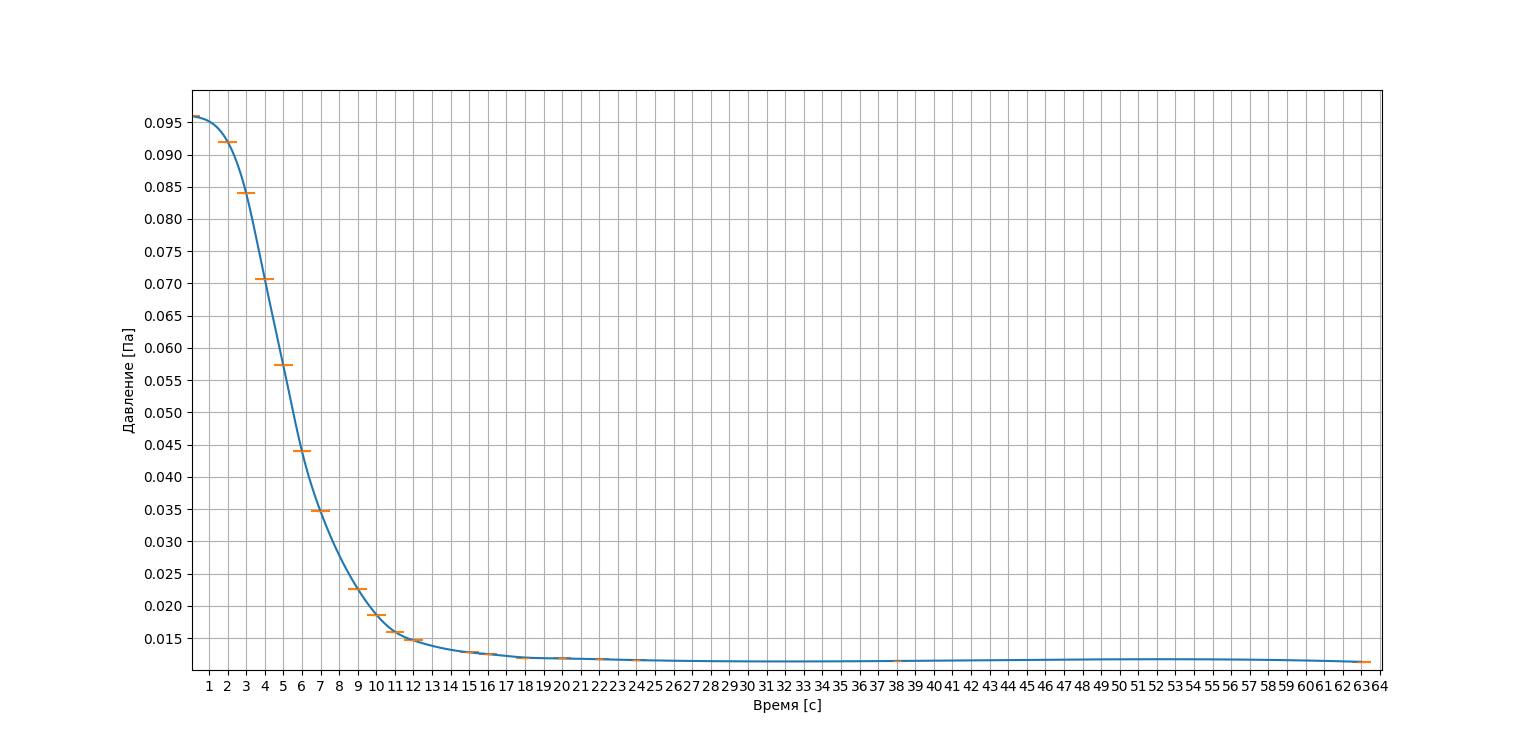
\includegraphics[scale = 0.3]{pressurebyTime.png} \\
Как видим, зависимость на участке 2-10 секунд напоминает экспоненциальную, что описывается формулой: 
\begin{equation}\label{PbyTime}
P = P_{0}\exp{-\frac{W}{V}\cdot t}+P_{limit}
\end{equation}
\\
, где $P_{0}$ - некотрое начальное значение давления, $W$ - скорость откачки, $P_{limit}$ - предельное значение давления
\\
После учаска экспоненциальной зависимости наблюдаем прямую, практически параллельную оси x. Значит в установке было достигнуто предельное давление, и коэффициент наклона $\alpha \xrightarrow[]{} 0$.

Убедимся в экспоненциальной зависимости на участке 2-10, и рассчитаем скорость откачки $W$. Для этого построим график в логарифмическом масштабе по оси $y$ и методом наименьших квадратов рассчитаем коэффициент наклона прямой:\\
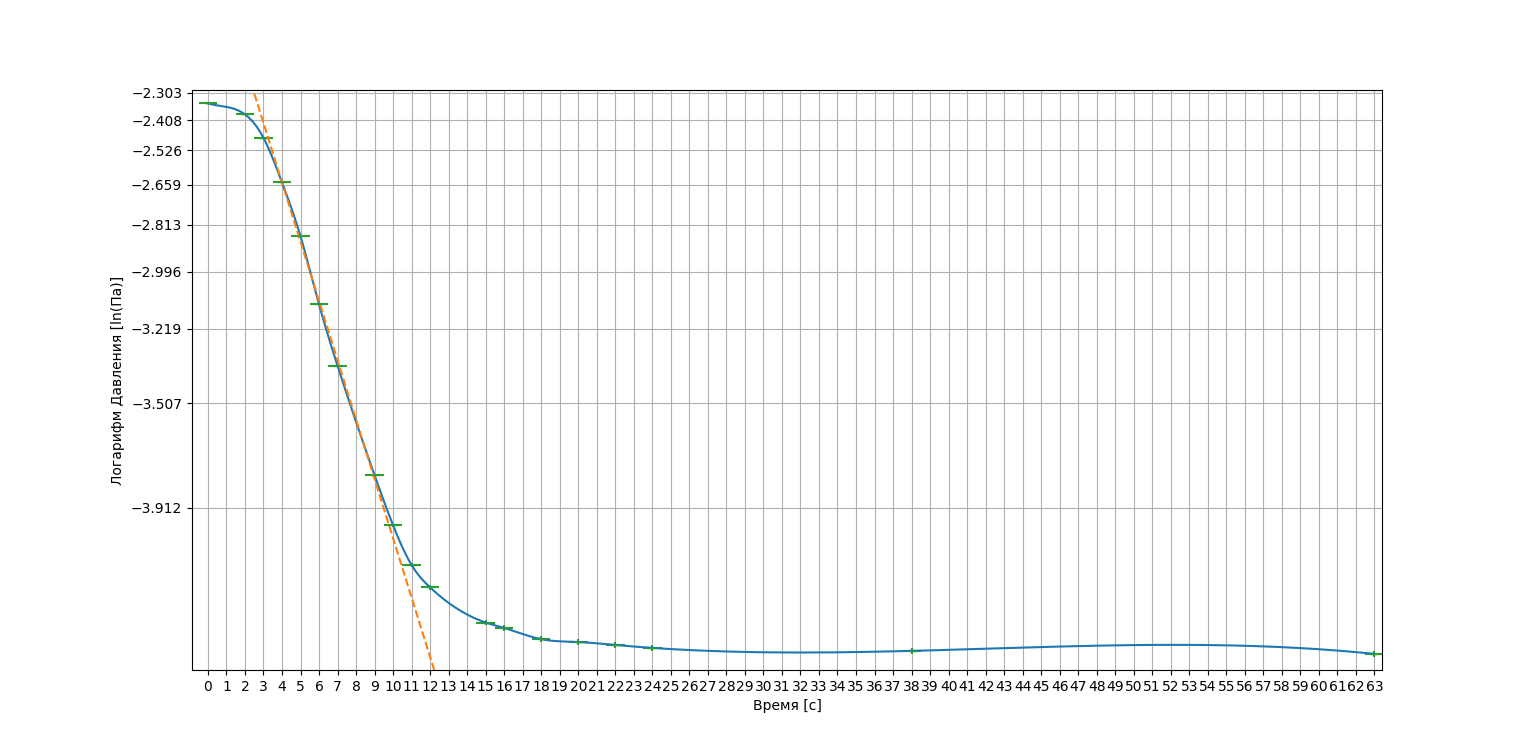
\includegraphics[scale = 0.3]{logPresurreByTime.png}
\begin{equation}
\alpha = -0.230 \pm 0.005
\end{equation}
Выразим сокрость откачки из формулы \eqref{PbyTime}:
\begin{equation}\label{difflnP}
    d\ln{P} = -\frac{W}{V}\cdot dt
\end{equation}
\begin{equation}\label{W}
    W = -\alpha V
\end{equation}
Получим $W = 0.80 \pm 0.04$ л/c
\subsection{Рассчитаем поток газа, поступающего из насоса в откачивающую систему}

Теперь потсроим график зависимости давления от времени при ухудшении вакуума, методом наименьших квадратов оценим коэффициенты наклона:
\begin{equation}
    \alpha = 1.09 \cdot 10^{-3} \pm 1 \cdot 10^{-5}
\end{equation}
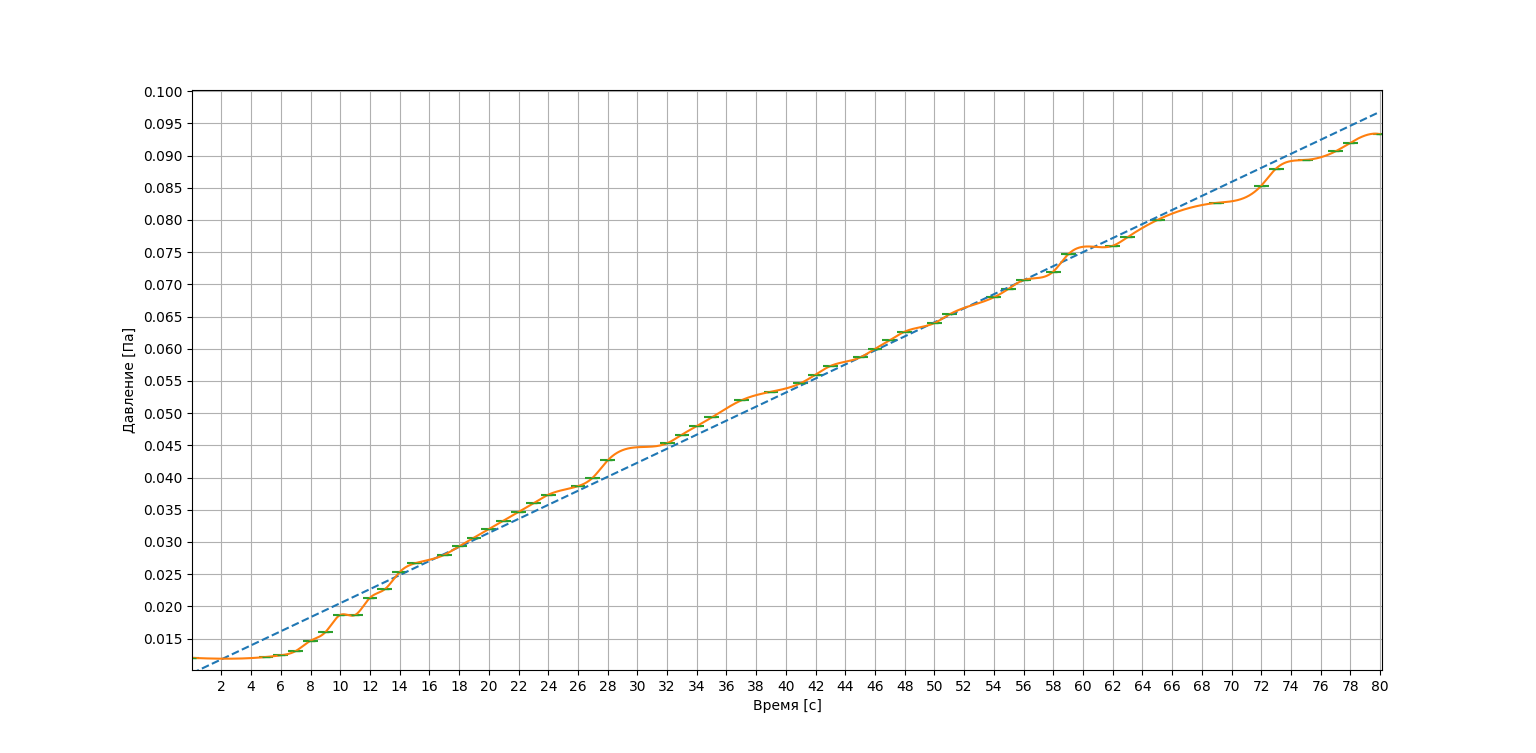
\includegraphics[scale = 0.3]{pressurebyTimeExp2.png}

Воспользуемся основным уравнением, описывающим процесс откачки. Учтем, что во время выполнения данной части эксперемента течей извне создано не было: $Q_{out} = 0$. Получим:
\begin{equation}
    Q_{p} = P_{limit}W - V_{hv} \alpha
\end{equation}
Методом частных производных оценим погешности, в результате получим значение:
$Q_{p} = 0.0073 \pm 0.0005$ Л*Па/с
\subsection{Измерение скорости откачки в условиях течи}


Воспользуемся формулами:
\begin{equation}
    P_{limit} W = Q_{1} 
\end{equation}
\begin{equation}
    P_{set} W = Q_{1}+\frac{d (P V)_{k}}{d t}
\end{equation}
Выразим $Q_{1}$ - сумму натеканий без учета натекания через искусственную течь. Подставив выраженное значение в формулу (6) и рассчитав количество газа, проходящего через каппиляр сможем рассчитать скорость откачки.

В результате получим: $W_{1} = 0.0560 \pm 0.0012$ л/с. 

\section{Вывод}


С точностью $5 \%$ удалось рассчитать скорость откачки. Скорость откачки во втором эксперименте меньше скорости откачки в первом примерно на $25 \%$. Очевидно, так как искусственная течь 'мешает' откачке. 

Об аккуратности проведения эксперимента и правильной работе оборудования можно судить по малому коэффициенту наклона графика зависимости $P(t)$ в эксперименте по ухудшению вакуума и малая масса газа потсупающая в установку через насос.

Предельное давление, полученное в эксперименте, составило порядка $8.3 \cdot 10^{-5}$ мм.рт.с, что соответсвует длине свободного пробега порядка нескольких дециметров. Такой вакуум классифицируется как <<высокий>>, так как равновероятно столкновение со стенками и с другими молекулами: $\lambda/d \approx 1$.
\end{document}